
\chapter{Exporting \pf models as FMUs}

The FMI specification requires all exported models to define a notion of time.
In \pf there are several ways to introduce such a notion of time within a model.
In the following, the ways supported by the \fmipp \pf FMU export library are presented.


Furthermore, a naming convention is needed that allows to refer to parameters defined in a \pf model in an FMI compliant way (e.g., in the model description).
For the \fmipp \pf FMU export utility this is done by concatenating a parameter's name with the associated object's type and name in the following way:
\begin{verbatim}
FMI compliant name = <object-type>.<object-name>.<parameter-name>
\end{verbatim}
For instance, the parameter \texttt{plini} associated to a general load (object type \texttt{ElmLod}) called \texttt{Load} would be referred to as \texttt{ElmLod.Load.plini} in the model description.

\section{Exporting models using triggers}

Parameters in \pf can be associated with a time series by providing an external file, called a \emph{Parameter Characteristic from File} (\pf object of type \texttt{ChaVecFile}).
The actual value of the parameter can be changed by associating a \emph{Trigger and Unit for File} (\pf object of type \texttt{TriFile}) to such a time series.
Figure~\ref{fig:characteristics_from_file} shows the setup window for such a characteristic from file, which defines the associated external file (called \texttt{TestTriggers-characteristics.csv}) and the trigger (defined via the \texttt{Scale} field).
Figure~\ref{fig:trigger_for_file} shows the setup for the trigger itself.

\begin{figure}[h!]
\centering{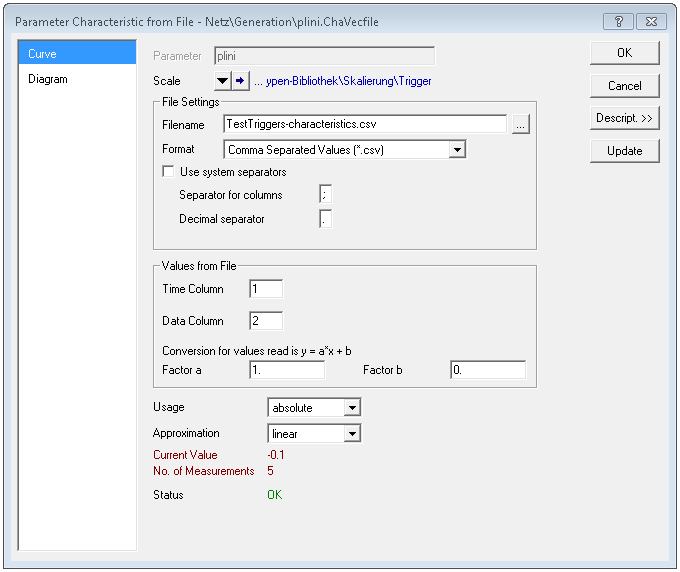
\includegraphics[width=0.9\textwidth]{characteristics_from_file}}
\caption{\pf window for defining a parameter characteristic from file.}
\label{fig:characteristics_from_file}
\vspace{1em}
\end{figure}

\begin{figure}[h!]
\centering{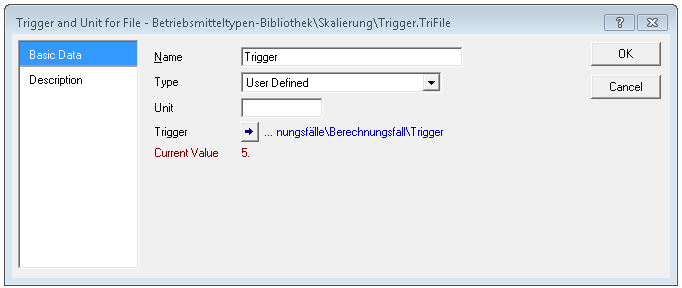
\includegraphics[width=0.85\textwidth]{trigger_for_file}}
\caption{\pf window for defining a trigger and unit for file.}
\label{fig:trigger_for_file}
\end{figure}

In order to create an FMU from a PFD file that defines characteristics from files and triggers, a \python script has to be executed from the command prompt window (please refer to the \href{https://docs.python.org/2/faq/windows.html}{\python~FAQ} in case you need assistance with this).
Open the command prompt window and execute the script \texttt{powerfactory\_fmu\_create.py}:

\begin{verbatim}
python <path_to_pf_fmu_dir>powerfactory_fmu_create.py [-h] [-v] 
  -m model_id -p pfd_file [-d pf_install_dir] [-i input_var_file]
  [-o output_var_file] [-t name:scale] [additional_file_1 ... ]
  [var1=start_val1 ...]
\end{verbatim}

The path to the installation directory of the \fmipp \pf FMU export utility \verb!<path_to_trnsys_fmu_dir>! may be relative or absolute.
Optional arguments are enclosed by squared brackets \verb![!$\,$\ldots\verb!]!, terms in angle brackets \verb!<!$\,$\ldots\verb!>! represent file paths.
  
\textit{Mandatory input arguments}:
  \begin{itemize}
    \item \verb!-m, --model-id!: specify FMU model identifier
    \item \verb!-p, --pfd-file!: path to PowerFactory PFD file
  \end{itemize}
  \textit{Optional input arguments}:
  \begin{itemize}
    \item \verb!-h, --help!: display the help screen
    \item \verb!-v, --verbose!: turn on log messages
    \item \verb!-l, --litter!: do not clean-up intermediate files
    \item \verb!-i, --input-var-file!: specify file containing list of input variable names
    \item \verb!-o, --output-var-file!: specify file containing list of output variable names
    \item \verb!-t, --trigger!: specify a trigger for advancing simulation time
    \item \verb!-d, --pf-install-dir!: path to \pf installation directory
  \end{itemize}
\end{enumerate}
Files containing lists of input and output variable names are expected to be in clear text, listing exactly one valid variable name per line.
As explained above, variable names are supposed to be of the  form \texttt{<object-type>.<object-name>.<parameter-name>}.

Triggers for simulation time advance need to be defined in the form \texttt{<name>:<scale>}.
The \texttt{name} has to be given according to the trigger's object name in the PFD file.
Times given to the FMU are interpreted as seconds, therefore the \texttt{scale} can be adjusted to match the trigger's internal unit of time (e.g., 60 for minutes or 3600 for hours).
Multiple triggers may be defined.

Additional files may be specified (e.g., CSV load profiles) that will be automatically copied to the FMU. The specified files paths may be absolute or relative.

Furthermore, start values for variables may be defined. For instance, to set a variable with the name \texttt{ElmLod.TestLoad.plini} to a value of 12.34, specifiy \texttt{ElmLod.TestLoad.plini=12.34} in the command line as optional argument.



\section{Exporting models using DPL scripts}



\begin{Verbatim}[frame=single,commandchars=\\\{\}]

  \codeHighlightGreen{! Change date/time of active study case,}
  \codeHighlightGreen{! using the hour of the year (as float).}
  \codeHighlightGreen{!}
  \codeHighlightGreen{! ATTENTION: The script doesn't properly}
  \codeHighlightGreen{! handle simulation runs longer than one}
  \codeHighlightGreen{! year.}

  \codeHighlightBlue{object} \textcolor{black}{set_time;}

  \textcolor{black}{set_time =} \codeHighlightBlue{GetCaseObject}\textcolor{black}{(} \codeHighlightRed{'SetTime'} \textcolor{black}{);}

  \codeHighlightBlue{if} \textcolor{black}{( set_time ) \{}
  \textcolor{black}{  set_time:min = 0.0;}
  \textcolor{black}{  set_time:sec = 0.0;}
  \textcolor{black}{  set_time.SetTime( hour_of_year );}
  \textcolor{black}{\}}

\end{Verbatim}
